\begin{surferPage}[Sextique de Barth]{La Sextique de Barth}
    Cette surface de degré $6$ (sextique) fut construite par Wolf Barth en 1996. 
    
    La Sextique de Barth a en tout $65$ singularités.
%    (wenn man die $15$ im Bild nicht sichtbaren, ``unendlich fernen'', mitzählt)%
   C'est le plus grand nombre possible de singularités sur une sextique, comme cela fut démontré
    par Jaffe et Ruberman peu après la construction de Barth. Ainsi, le record de Barth
    est imbattable !


    La construction de Barth fut une grande surprise car il fut longtemps cru
    que les surfaces de degré $6$ devaient avoir au plus $64$ singularités.

   Une propriété remarquable de cette construction est sa symétrie icosaédrale; 
    la figure illustre un icosaèdre et ses plans de symétrie :  
%    Die Abb.\ zeigt diesen platonischen Körper und seine Symmetrie - Ebenen: 
%    und diese Ebenen gemeinsam mit der Barth Sextik in einem Bild.     
    % 
  \begin{center}
      \vspace*{-0.1cm}
      \begin{tabular}{@{}c@{\ \ }c@{\,}c@{}}
        \begin{tabular}{@{}c}
          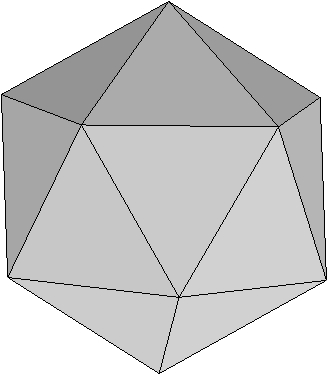
\includegraphics[width=1.4cm]{./../../common/images/icosah}
        \end{tabular}
        &
        \begin{tabular}{@{}c}
          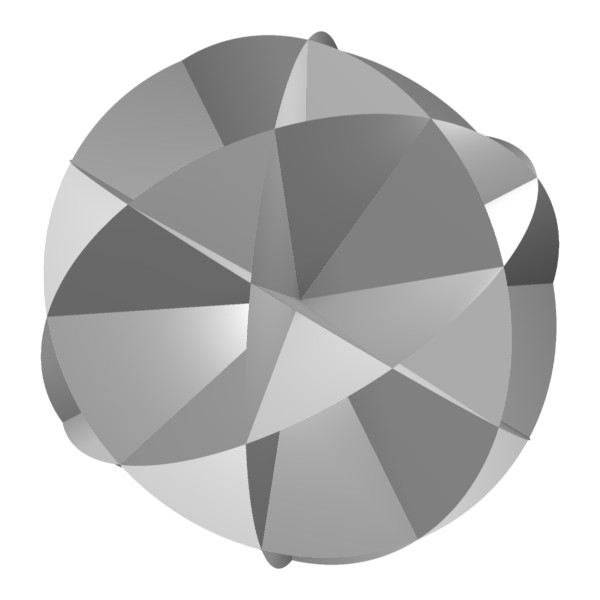
\includegraphics[width=1.4cm]{./../../common/images/barth_sextic_planes}
        \end{tabular}
        &
        \begin{tabular}{c@{}}
          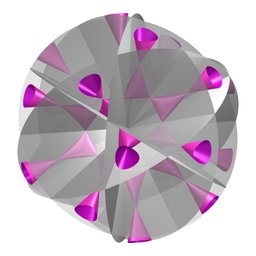
\includegraphics[width=1.4cm]{./../../common/images/barth_sextic_and_planes}
        \end{tabular}
      \end{tabular}
    \end{center}
    \vspace*{-0.1cm}

    La Sextique de Barth satisfait l'équation 
    $P_6 - \alpha K^2=0,$ où $P_6$
    renvoie aux 
    six plans de symétrie, $K=x^2+y^2+z^2-1$ est la sphère unité et 
    $\alpha=\frac{1}{4}(2+\sqrt{5})$.
\end{surferPage}
